\documentclass[slides,compress]{beamer}
\usepackage{graphicx,amsmath,hyperref}
\usepackage{verbatim}

\usepackage[normalem]{ulem}

\usetheme{default}
\useinnertheme{rectangles}

\title{\huge xia2 \& pipelines}
\subtitle{\large CCP4 developers meeting 2012}

\author{Graeme Winter}
\institute{Diamond Light Source}
\date{21 March 2012}

\begin{document}

\setbeamertemplate{background}{

\includegraphics[width=\paperwidth,height=\paperheight]
{diamond-background.png}
}

\frame{\maketitle}

\frame{
\frametitle{Overview}
\begin{itemize}
\item{xia2 developments}
\item{Removal of frame count limitations}
\item{Current state of multi-crystal analysis}
\item{Plans for multi-crystal analysis}
\item{Fast EP}
\end{itemize}
}

\frame{
\frametitle{xia2 developments}
\begin{itemize}
\item{xia2 for small molecule data reduction using XDS}
\item{Bugs / fixes}
\item{Using Aimless}
\item{\sout{P1 integration}}
\item{\sout{Scaling XDS data with Scala / Aimless}}
\end{itemize}
}

\frame{
\frametitle{Removal of frame count limitations}
\begin{itemize}
\item{Use Aimless in place of Scala}
\item{Use Pointless in place of Reindex\footnote{This is still not as
      efficient as it could be - but it works}}
\item{Run -3daii or -3da}
\item{No more batch limitations}
\end{itemize}
}

\frame{
\frametitle{Plate data}
\begin{itemize}
\item{Data from Diamond I04-1}
\item{110 x 100 image sweeps (20 degree)}
\item{Processed with xia2 -3daii -failover -spacegroup ... -cell ...}
\item{... crashed (this is to be expected!)}
\item{In XSCALE output analyse $CC(i,j)$, scale to $d = \frac{1}{CC} -
    1$ - useful distances}
\item{Get dendogram}
\end{itemize}
} 

\frame{
\frametitle{Results}
\begin{center}
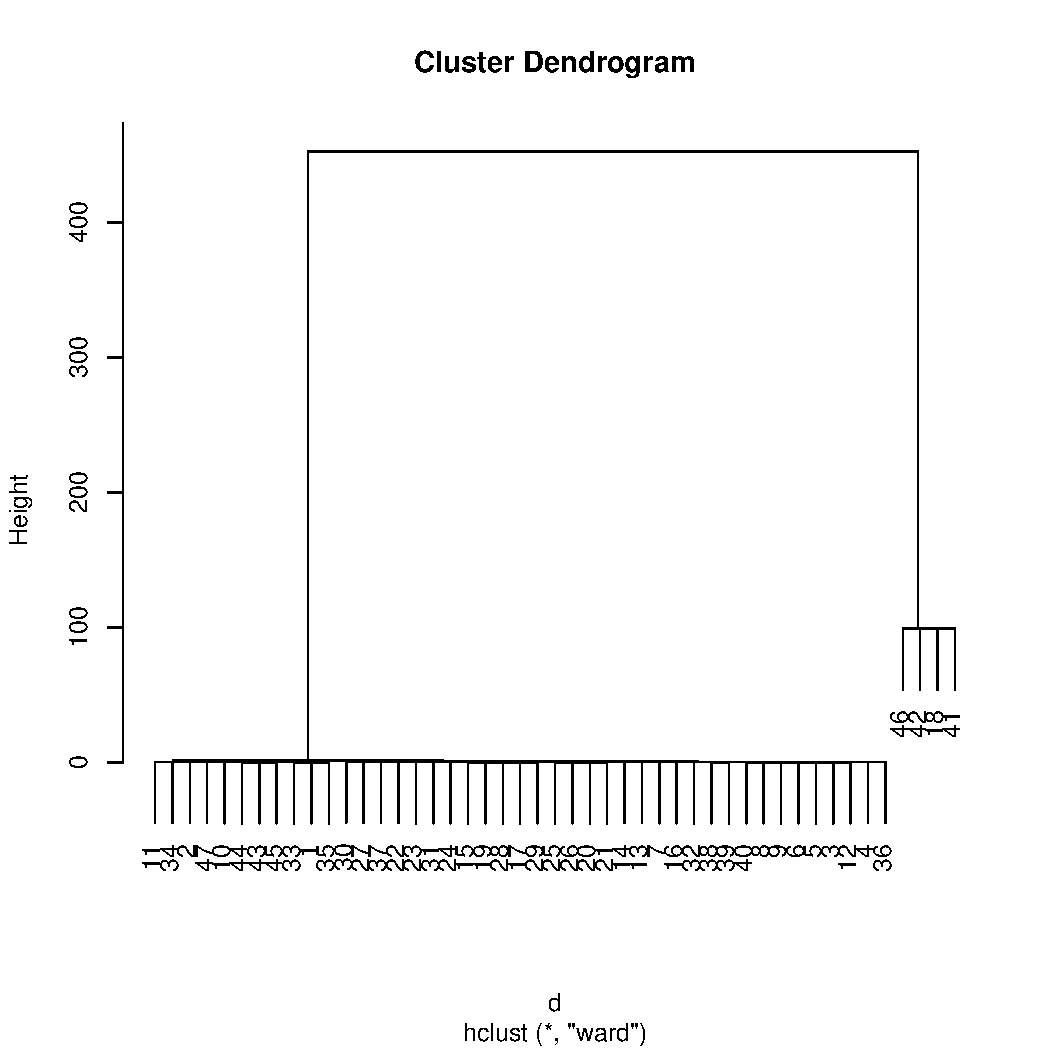
\includegraphics[scale=0.35]{L1.pdf}
\end{center}
}

\frame{
\frametitle{Next steps}
\begin{itemize}
\item{Remove useless sweeps, run again}
\item{This process is partially automated}
\item{xia2 -3daii (etc.) -xinfo mod.xinfo}
\item{Runs now to completion}
\end{itemize}
}

\begin{frame}[fragile]
\begin{verbatim}
For AUTOMATIC/DEFAULT/NATIVE
High resolution limit     1.77	  7.93	  1.77
Low resolution limit     39.42	 39.42	  1.82
Completeness          	 88.7	 99.5	 19.7
Multiplicity          	 39.2	 46.8	  1.8
I/sigma               	 21.0	 35.1	  3.1
Rmerge                	0.275	0.261	0.204
Rmeas(I)              	0.279	0.264	0.281
Rmeas(I+/-)           	0.280	0.265	0.268
Rpim(I)               	0.037	0.039	0.168
Rpim(I+/-)            	0.049	0.047	0.172
Wilson B factor       	22.655
Total observations    	429848	8325	318
Total unique          	10962	178	174
\end{verbatim}
\end{frame}

\frame{
\frametitle{Results}
\begin{center}
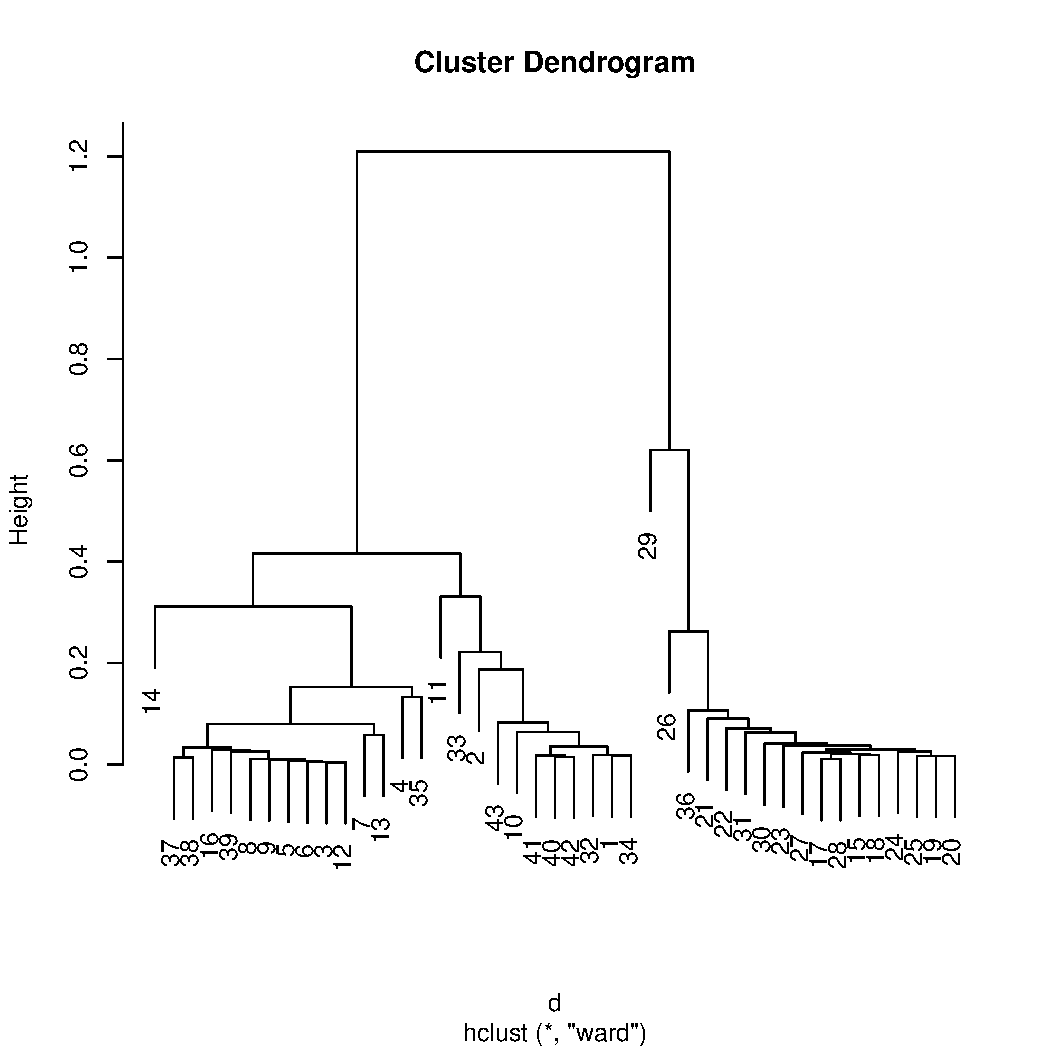
\includegraphics[scale=0.35]{L2.pdf}
\end{center}
}

\frame{
\frametitle{Cluster 1: 37, 38, 16, 39, 8, 9, 5, 6, 3, 12}
\begin{itemize}
\item{Use Re-Xinfo to take selected runs from dendogram, x1335 output
    and automatic.xinfo to generate new xinfo}
\item{... and run \emph{again}}
\end{itemize}
}

\begin{frame}[fragile]
\begin{verbatim}
High resolution limit     1.74	  7.79	  1.74
Low resolution limit     39.42	 39.42	  1.79
Completeness          	 84.2	 93.4	 16.3
Multiplicity          	 11.2	 12.3	  1.5
I/sigma               	 17.4	 31.9	  2.5
Rmerge                	0.099	0.068	0.213
Rmeas(I)              	0.105	0.072	0.334
Rmeas(I+/-)           	0.105	0.072	0.292
Rpim(I)               	0.026	0.019	0.211
Rpim(I+/-)            	0.034	0.022	0.199
Wilson B factor       	22.448
Total observations    	121810	2097	237
Total unique          	10858	170	153
\end{verbatim}
\end{frame}

\frame{
\frametitle{Results}
\begin{center}
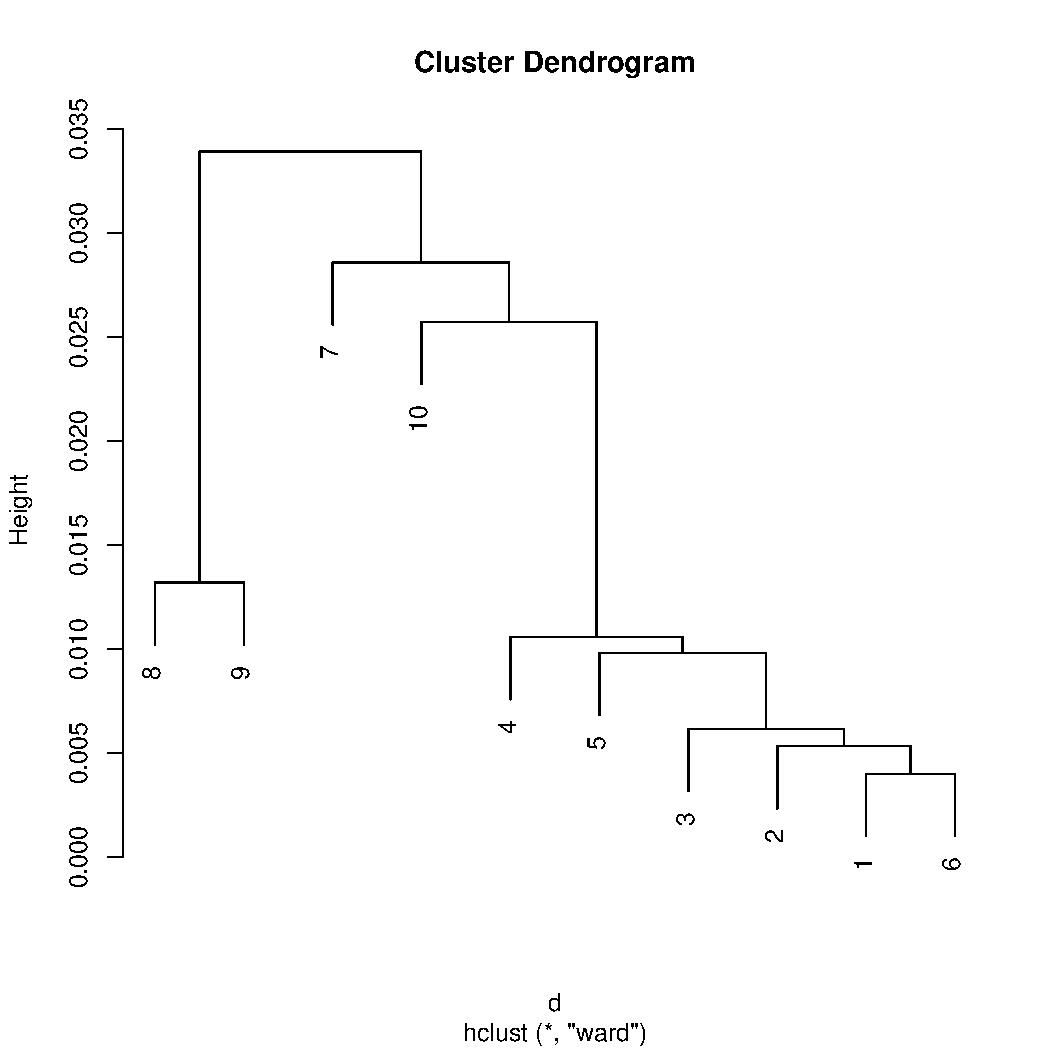
\includegraphics[scale=0.35]{cluster1.pdf}
\end{center}
}

\frame{
\frametitle{Results}
\begin{center}
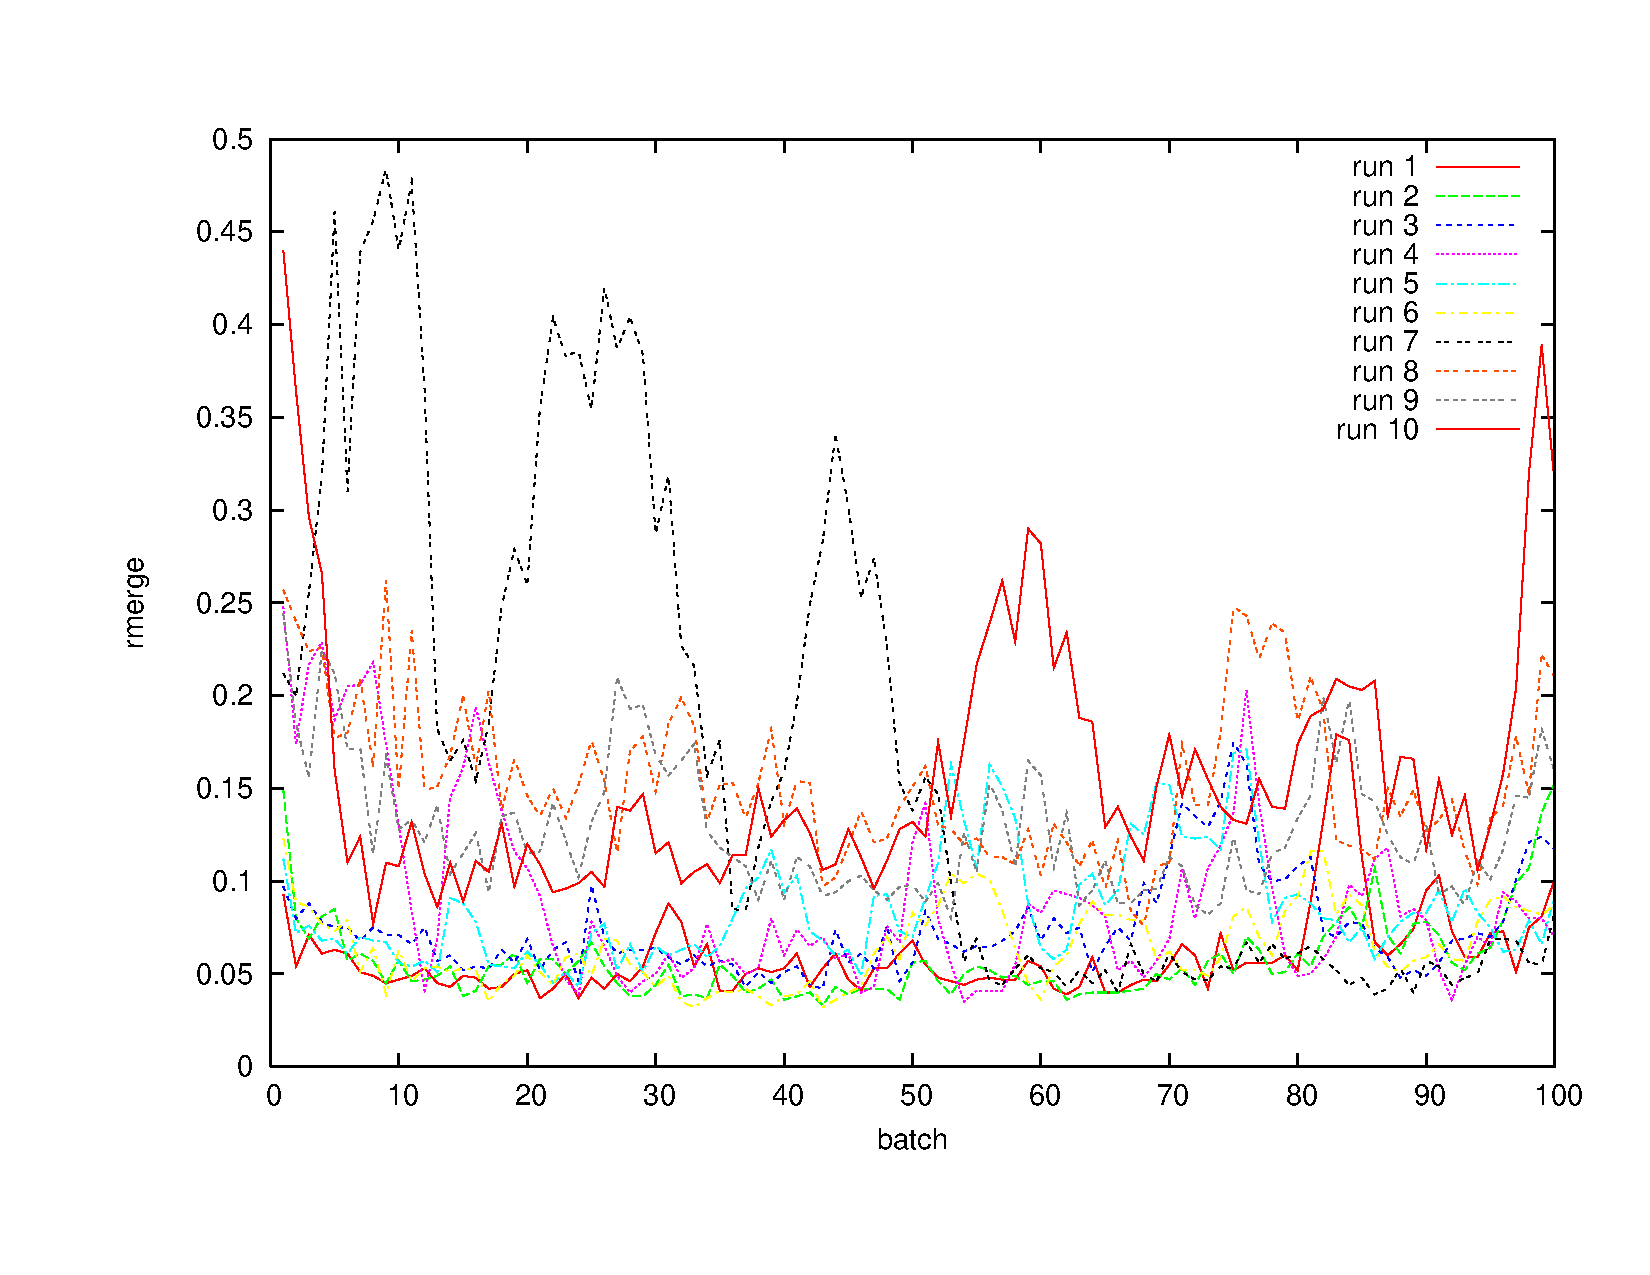
\includegraphics[scale=0.35]{Rmerge.pdf}
\end{center}
}

\frame{
\frametitle{Next steps: April 2012 onwards}
\begin{itemize}
\item{Automate this procedure, allow user to specify requirements}
\item{Include BLEND analysis: complementary information}
\item{Code up own $CC$ calculation: can run from Aimless output}
\item{Automate $R_{\rm{merge}}$ \emph{vs.} BATCH \emph{vs.} run
    analysis}
\end{itemize}
}

\frame{
\frametitle{Fast EP}
\begin{itemize}
\item{Experimental phasing in the spirit of Fast DP}
\item{Uses shelxc / d\_mp / e}
\item{Extentive use of CCTBX for analysis}
\item{Can give maps within 2 minutes of experiment in favourable cases
    - DP 1 minute, EP 1 minute}
\item{Takes no information, searches everything (spacegroups, sites, hands)}
\end{itemize}
}

\frame{
\frametitle{Brute force / power}
\begin{itemize}
\item{Assess with CCTBX code}
\item{Use shelxc to get ins file, hkl file}
\item{Modify using CCTBX}
\item{Run shelxd\_mp on cluster: up to 480 x 3GHz cpu's}
\item{Sort results on CFOM, find best, get number sites}
\item{Run 22 shelxe runs: 2 hands, 11 solvent fractions, score on
    pseudo-free $CC$}
\end{itemize}
}

\end{document}
